\begin{figure}[htpb]
\centering\capstart{}
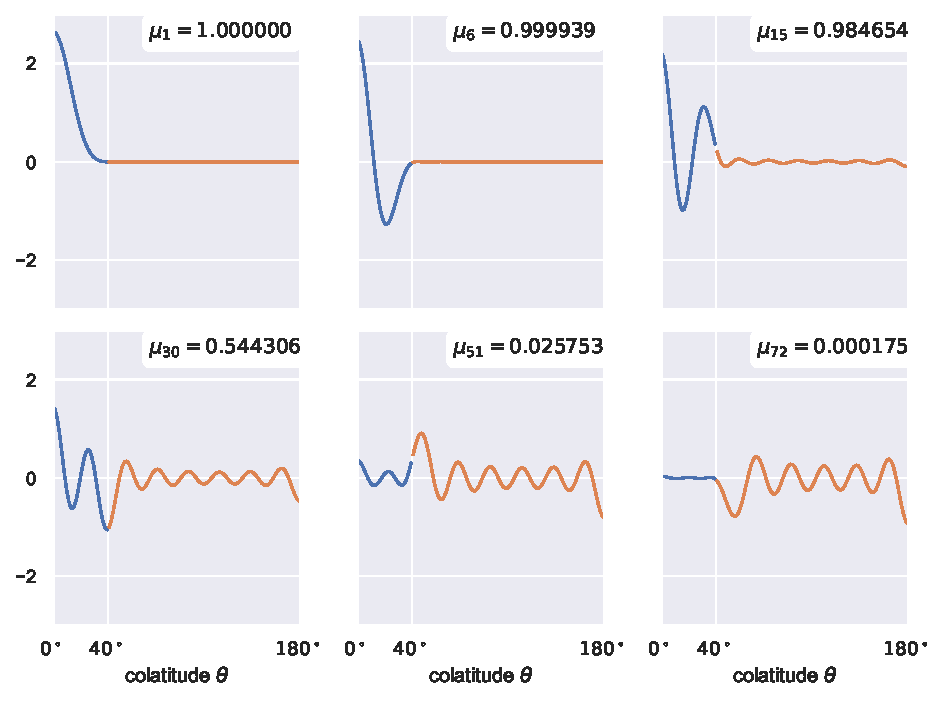
\includegraphics[width=\textwidth]{slepian_colatitude.pdf}
\caption[
The colatitudinal dependence of the polar cap Slepian functions
]{
The colatitudinal dependence of the Slepian functions \(\pixel{\slepian{S}}\) within a polar cap of colatitudinal radius \(\theta_{0}=\SI{40}{\degree}\) for \(p \in \set{1, 6, 15, 30, 51, 72}\) shown left-to-right, top-to-bottom.
The bandlimit here is  \(L=16\), which corresponds to a Shannon number of \(N=30\), \ie{} the final two panels are beyond the Shannon number.
Blue curves show the concentration within the cap \(\SI{0}{\degree} \leq \theta \leq \theta_{0}\), whilst orange curves show the leakage into the rest of the sphere \(\theta_{0} < \theta \leq \SI{180}{\degree}\).
The eigenvalue \(\slepian{\mu}\) quantifies the relative spatial concentration of the Slepian function, where lower values have increasing leakage into the orange curve.
}\label{fig:chapter2_slepian_colatitude}
\end{figure}
